\chapter{Other Plots}\label{sec:other_plots}

\section{Signal Fits in \texorpdfstring{$m_{KK}$}{mKK}}

\begin{figure}[H]
	\centering
	\captionsetup{width=0.8\linewidth}
	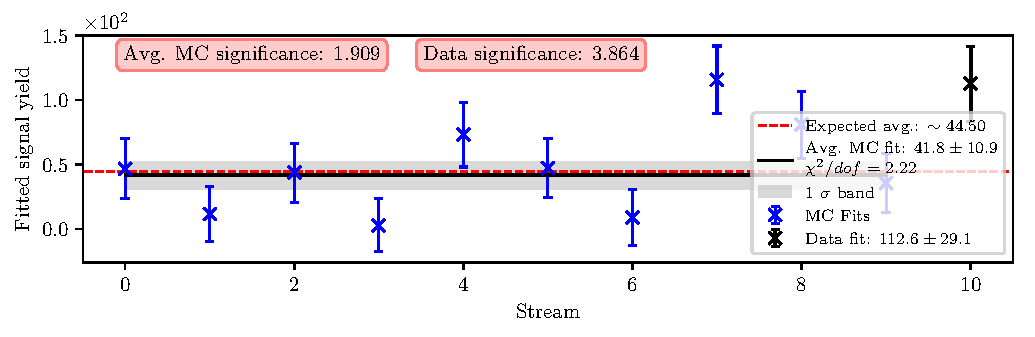
\includegraphics[width=\linewidth]{fig/sig_mKK_1}
	\caption{Signal fit result for the $1^{\mathrm{st}}$ $m_{KK}$ window for MC and data in the range $0.980  < m_{KK} < 1.011$.}
\end{figure} 

\begin{figure}[H]
	\centering
	\captionsetup{width=0.8\linewidth}
	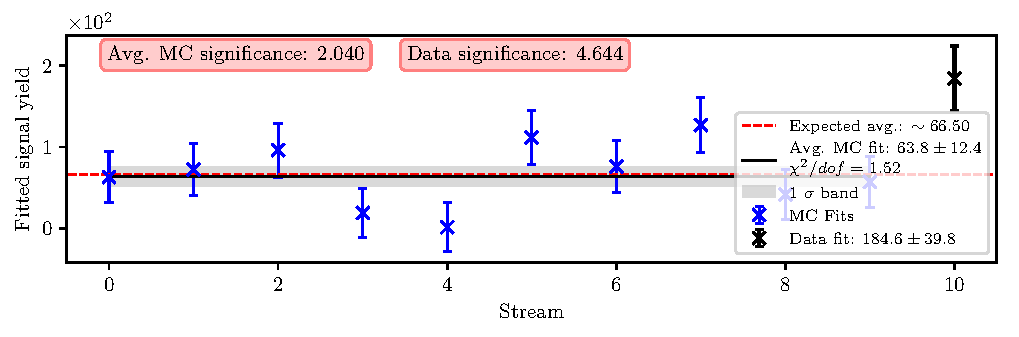
\includegraphics[width=\linewidth]{fig/sig_mKK_2}
	\caption{Signal fit result for the $1^{\mathrm{nd}}$ $m_{KK}$ window for MC and data in the range $1.011  < m_{KK} < 1.027$.}
\end{figure}

\begin{figure}[H]
	\centering
	\captionsetup{width=0.8\linewidth}
	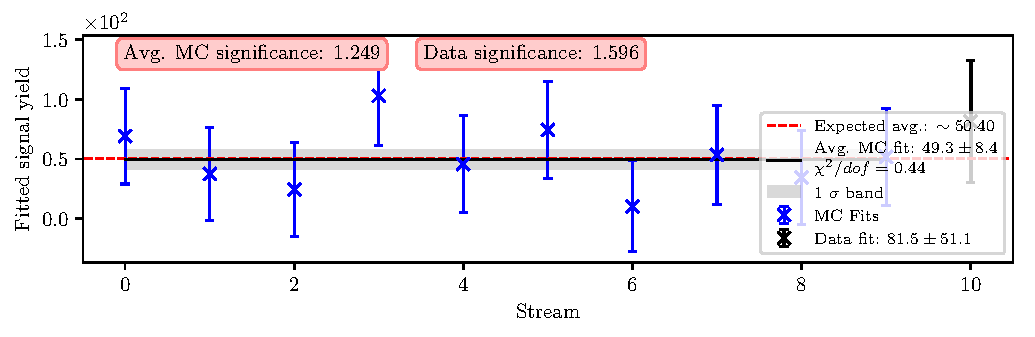
\includegraphics[width=\linewidth]{fig/sig_mKK_3}
	\caption{Signal fit result for the $1^{\mathrm{rd}}$ $m_{KK}$ window for MC and data in the range $1.027  < m_{KK} < 1.187$.}
\end{figure}

\begin{figure}[H]
	\centering
	\captionsetup{width=0.8\linewidth}
	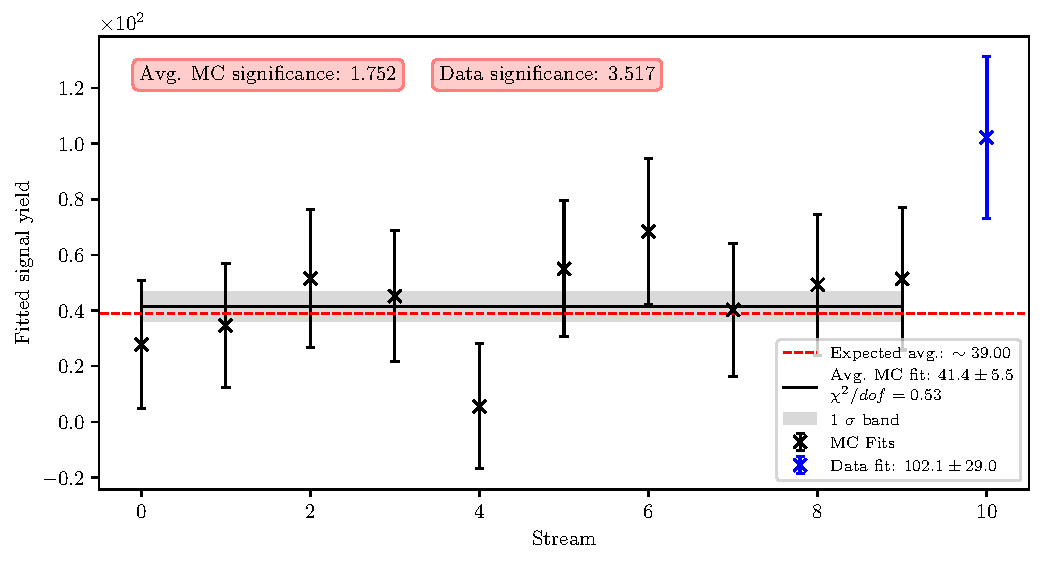
\includegraphics[width=\linewidth]{fig/sig_mKK_4}
	\caption{Signal fit result for the $1^{\mathrm{th}}$ $m_{KK}$ window for MC and data in the range $1.187  < m_{KK} < 1.342$.}
\end{figure}

\begin{figure}[H]
	\centering
	\captionsetup{width=0.8\linewidth}
	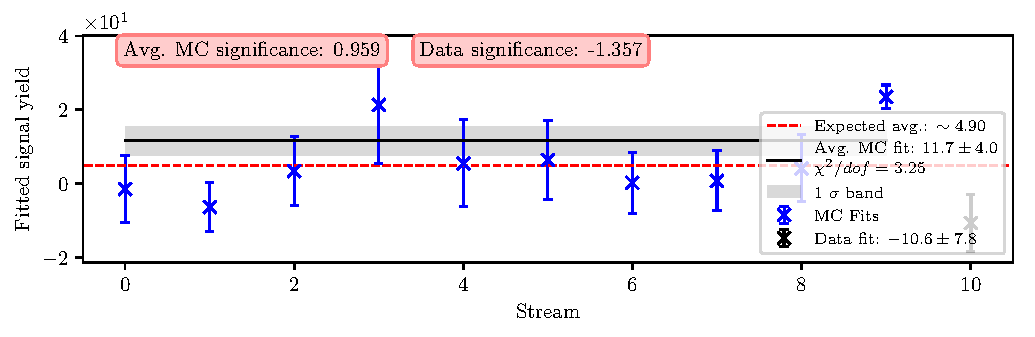
\includegraphics[width=\linewidth]{fig/sig_mKK_5}
	\caption{Signal fit result for the $1^{\mathrm{th}}$ $m_{KK}$ window for MC and data in the range $1.342  < m_{KK} < 1.497$.}
\end{figure}

\begin{figure}[H]
	\centering
	\captionsetup{width=0.8\linewidth}
	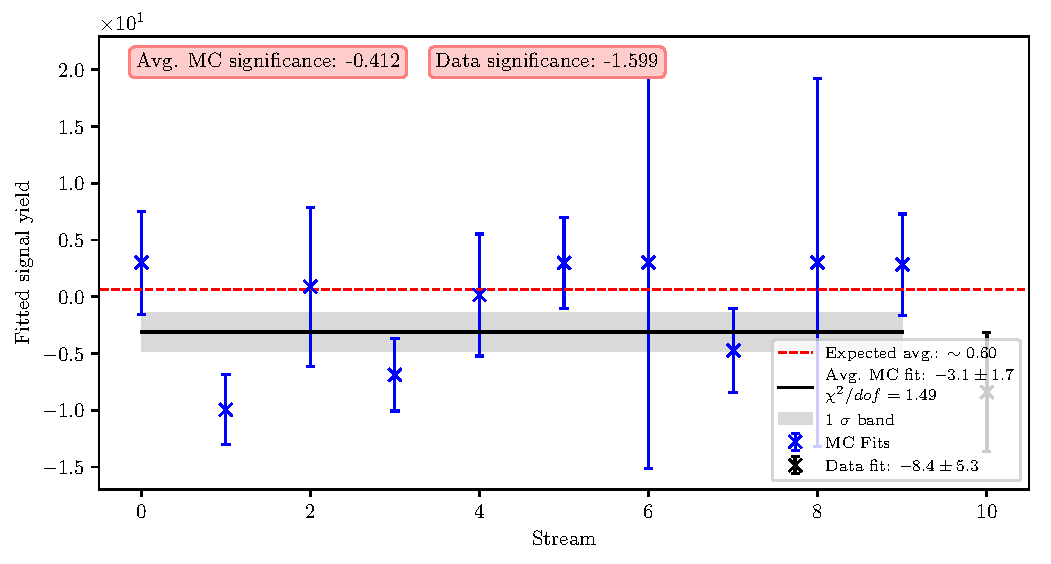
\includegraphics[width=\linewidth]{fig/sig_mKK_6}
	\caption{Signal fit result for the $1^{\mathrm{th}}$ $m_{KK}$ window for MC and data in the range $1.497  < m_{KK} < 1.647$.}
\end{figure}

\begin{figure}[H]
	\centering
	\captionsetup{width=0.8\linewidth}
	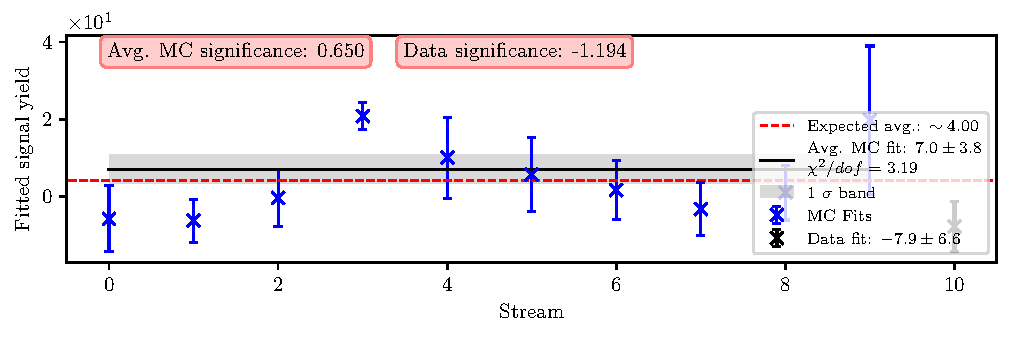
\includegraphics[width=\linewidth]{fig/sig_mKK_7}
	\caption{Signal fit result for the $1^{\mathrm{th}}$ $m_{KK}$ window for MC and data in the range $1.647  < m_{KK} < 1.850$.}
\end{figure}

\begin{figure}[H]
	\centering
	\captionsetup{width=0.8\linewidth}
	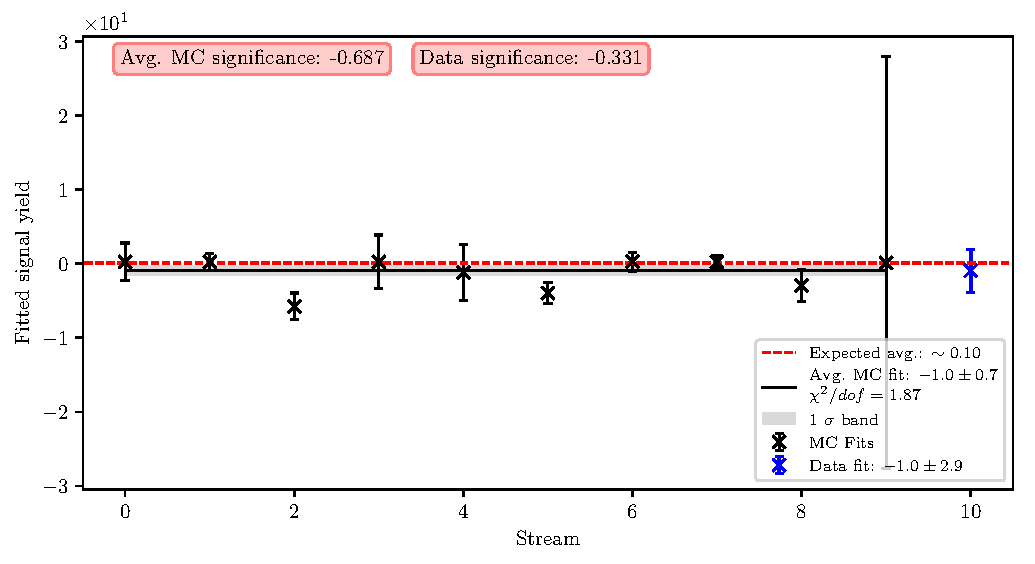
\includegraphics[width=\linewidth]{fig/sig_mKK_8}
	\caption{Signal fit result for the $1^{\mathrm{th}}$ $m_{KK}$ window for MC and data in the range $1.850  < m_{KK} < 1.880$.}
\end{figure}

\begin{figure}[H]
	\centering
	\captionsetup{width=0.8\linewidth}
	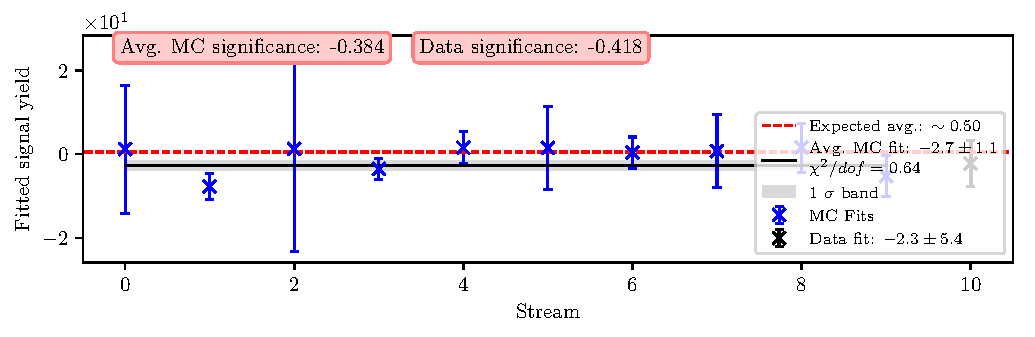
\includegraphics[width=\linewidth]{fig/sig_mKK_9}
	\caption{Signal fit result for the $1^{\mathrm{th}}$ $m_{KK}$ window for MC and data in the range $1.880  < m_{KK} < 3.660$.}
\end{figure}